\documentclass[12pt]{scrartcl} %or scrbook

\usepackage{xcolor}
\definecolor{darkred}{rgb}{0.75,0,0}
\definecolor{darkblue}{rgb}{0,0,0.5}
\definecolor{darkgreen}{rgb}{0,0.5,0}
\definecolor{darkergreen}{rgb}{0,0.75,0}
\definecolor{darkmagenta}{rgb}{0.55,0,0.55}
\definecolor{left}{HTML}{041832}
\definecolor{secondary}{HTML}{241024}
\usepackage{verbatim}
\usepackage{graphicx}
\usepackage[export]{adjustbox}
\usepackage[colorlinks=true,
		     urlcolor=darkblue,
		     citecolor=darkergreen,
		     linkcolor=darkblue,
		     plainpages=false,
		     pdfpagelabels]{hyperref}

\setlength{\parindent}{0pt}
\setlength{\parskip}{.25cm}

\usepackage{graphicx}

%If you want to typeset code, use minted (requires
%some additional setup)
\usepackage{minted}

%If you want to typeset algorithms, use algorithm2e:
\usepackage[boxed,slide,linesnumbered]{algorithm2e}

\title{BumprCars Invoicing}
\subtitle{Computer Science II}
\author{Casey Nolte\\
        \href{mailto:casey.nolte@huskers.unl.edu}{casey.nolte@huskers.unl.edu} \\
        Jack Kieny\\
        \href{jackkieny@huskers.unl.edu}{jackkieny@huskers.unl.edu} \\
        Department of Computer Science \& Engineering\\
        University of Nebraska---Lincoln\\
}

\date{Fall 2020 \\
      Version 1.0
}

\begin{document}

\maketitle
\thispagestyle{empty}

\vfill

\begin{abstract}
This document provides information regarding the design and function of BumprCars Invoicing. The purpose of Semester Project is to parse flat data files and produce more usable and user friendly data output. 
\end{abstract}

\newpage
\clearpage
\setcounter{page}{1}
\section*{Revision History}

\begin{tabular}{|l|l|l|l|}
\hline
Version & Description of Change(s) & Author(s) & Date \\
\hline
1.0 & Initial draft of this design document & Casey Nolte, Jack Kieny & 09/26/2020 \\
\hline
\end{tabular}

\newpage
\tableofcontents

\newpage
\section{Introduction}

%This document is an overview of BumprCars Invoicing. BumprCars Invoicing is a program in development for BumprCars, a business providing a multitude of products to many customers. 
%Provide a short introduction to this document, the project and the context in which it is being developed.  This document needs to conform to the 
%IEEE 1016 standard \cite{IEEE1016} (this is how you use citations).

\subsection{Purpose of this Document}

This document serves as an in depth description of the BumprCars Invoicing program and it's functionality. With sufficient understanding of this design document, a proficient programmer would be able to recreate the general function of this program. 
%Describe the purpose of this document; the goal(s) that its content are intended to achieve

\subsection{Scope of the Project}

In it's current iteration, BumprCars Invoicing includes functionality for the parsing of flat data files of persons, customers, and products, and then generating json files from these flat files. The program is also capable of reading a flat invoice file and generating a summary report as well as detailed individual reports. This program was developed to replace the outdated invoicing system at BumprCars, as a more modern object oriented solution provides better functionality. Not included currently in the project scope is database systems. 

%Describe the scope of the project, what features and functionality it covers (at a high-level).  Describe the problem statement and context in which this project is being developed.  Who is it for, what is it for, etc.?  You may also explicitly indicate what is not within the scope--other potential pieces of the overall project that are not covered by this document

\subsection{Definitions, Acronyms, Abbreviations}

\subsubsection{Definitions}

\begin{description}
  \item[Flat File] Non-standard data file
\end{description} 

%\subsubsection{Abbreviations \& Acronyms}

%[Define all abbreviations and acronyms used in this document here.  This relieves you of the need to define such things within the context of the document itself and provides an easy reference for the reader.]

%\begin{description}
%  \item[ACM] Association for Computing Machinery
%  \item[IEEE] Institute of Electrical and Electronics Engineers
%  \item[UAV] Unmanned Aerial Vehicle
%\end{description}
  
\section{Overall Design Description}
 Currently, BumprCars Invoicing contains classes for the storage of multiple different types of data, and methods for parsing data files and creating more user friendly data output. 
%[Provide an overall summary/description of the project.  Identify the major design components, technologies, etc.]
  
\subsection{Alternative Design Options}
At the moment, significant alternative options have not been discussed.
%If applicable, describe and discuss alternative design options that you considered and discuss why they were not chosen.  What advantages and disadvantages do the alternatives provide and what advantage/disadvantages do the chosen design elements provide.  Provide some justification for why the chosen elements? advantages/disadvantages outweighed the alternatives

\section{Detailed Component Description}

This section will detail multiple aspects of the BumprCars Invoicing system. Currently, it contains information about the class layout of the program. 

%\subsection{Database Design}

%This section will be used to detail your database schema design (Phase III).  In earlier phases this section may be omitted or a short note indicating that details will be provided in a subsequent revision of this document.

%\subsubsection{Component Testing Strategy}

%This section will describe your approach to testing this particular component.]

\subsection{Class/Entity Model}

In the BumprCars Invoicing program, the invoice, person, customer, and product classes each hold data of their respective type. Additionally, the product class is a superclass for repair, rental, towing, and concession classes. The FlatParser class contains methods used to parse flat data files and create instances of the data classes. The address class is used in the construction of the person class, and the person class is used in the construction of the customer class. The DataConverter class contains a main method that takes raw input files. See \ref{figure:classdiagram} for a visual representation of the class layout. 

%[This section should detail your Java classes--their state, interface and how they relate to each other.  It is highly recommended that you document these elements using tables, UML diagrams, and other visually-informative methods.  Figures and tables should have proper captions and be referenced in the main text just like in Figure \ref{figure:designDocument.png}.  You should provide subsections to organize your presentation as applicable.]

\begin{figure}[!h]
\centering
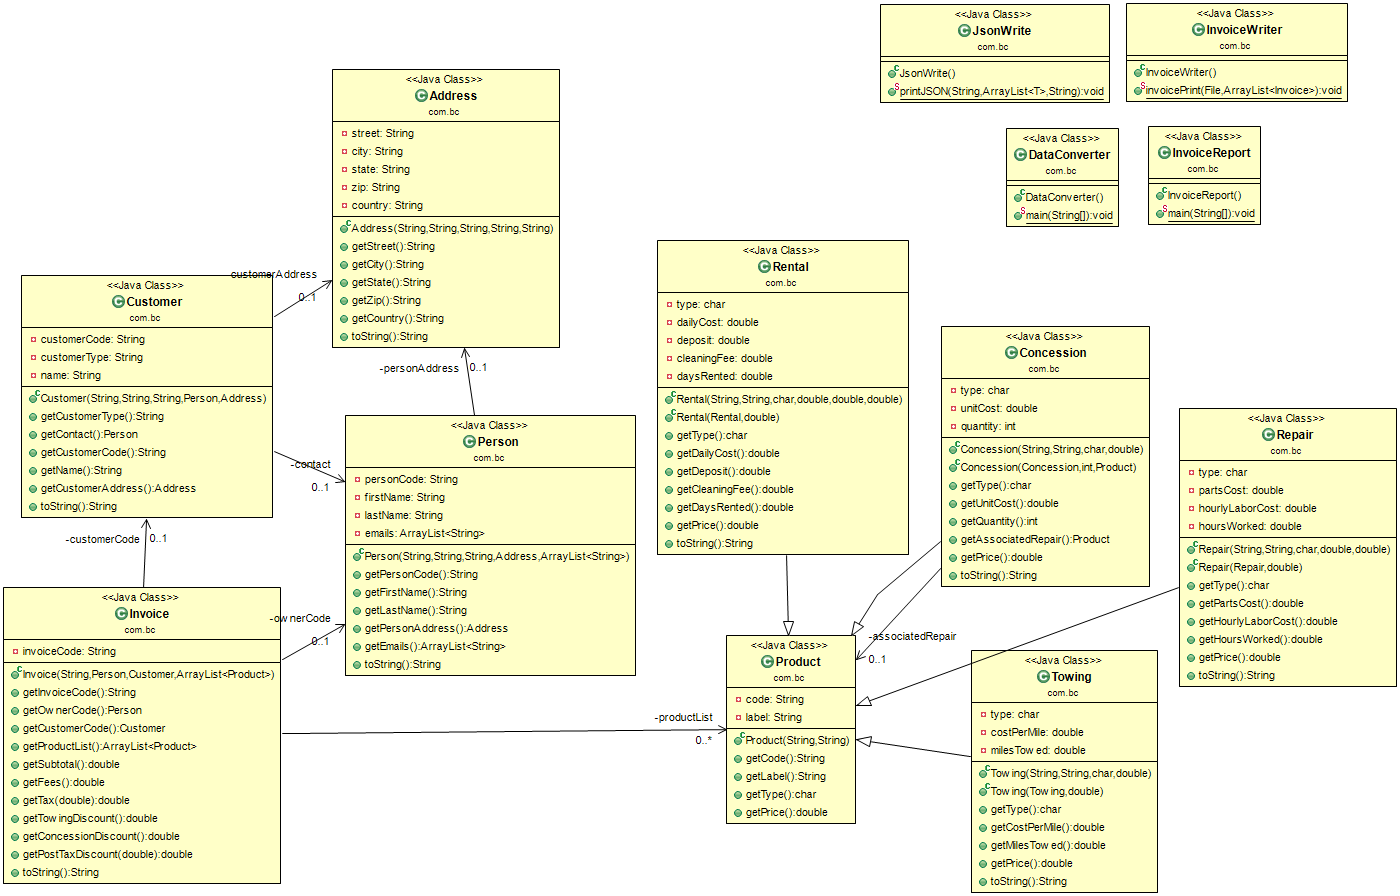
\includegraphics[max size={\textwidth}{\textheight}]{ClassDiagram.png}
\caption{Class Diagram for BumprCars Invoicing}
\label{figure:classdiagram}
\end{figure}

\subsubsection{Component Testing Strategy}

A multitude of test cases were run after phase 1 of the project that tested that parsing and saving of data from flat files, as well as the creation of json files. These test cases resulted in changes to the parsing system in order to deal with changing amounts of emails in the flat files. 
%This section will describe your approach to testing this particular component.  Describe any test cases, unit tests, or other testing components or artifacts that you developed for this component.  What were the outcomes of the tests?  Did the outcomes affect development or force a redesign?]

%\subsection{Database Interface}

%[This section will be used to detail phase IV where you modify your application to read from a database rather than from flat files.  This section will detail the API that you designed--how it conformed to the requirements, how it worked, other tools or methods that you designed to assist, how it handles corner cases and the expectations or restrictions that you?ve placed on the user of the API.  In earlier phases this section may be omitted or a short note indicating that details will be provided in a subsequent revision of this document.  An example table is presented
%as Table \ref{table:assignmentPerformance}.]

\begin{comment}
\begin{table}
\centering
\caption{Average Performance on Assignments; on-time vs. late and individual vs partners.  In general, captions for Tables should appear above the table.}
\label{table:assignmentPerformance}
\begin{tabular}{|l|p{1.5cm}|p{1.5cm}|p{1.5cm}|p{1.5cm}|p{1.5cm}|p{1.5cm}|p{1.5cm}|}
\hline
~ & 1 & 2 & 3 & 4 & 5 & 6 & 7 \\
\hline
On-time	& 93.16\% (78.46\%)	& 88.06\% (72.31\%)	& 87.89\% (67.69\%)	& 89.37\% (56.92\%) & 83.42\% (29.23\%) & 88.40\% (53.85\%) & 74.56\% (75.38\%) \\
\hline
Late & 88.75\% (12.31\%) & 85.28\% (20.00\%) & 70.32\% (15.38\%) & 90.40\% (15.38\%) & 82.74\% (44.62\%) & 94.22\% (15.38\%) & N/A \\
\hline
Diff & \color{red}{4.42\%} & \color{red}{2.79\%} & \color{red}{17.57\%} & \color{green}{1.03\%} & \color{red}{0.68\%} & \color{green}{5.82\%} & - \\
\hline
Individual & NA	& 88.43\% (73.85\%) & 82.32\% (33.85\%) & 87.22\% (27.69\%) & 86.40\% (23.08\%) & 82.67\% (26.15\%) & ~\\
\hline
Pairs & NA & 83.55\% (18.46\%) & 86.22\% (49.23\%) & 91.00\% (46.15\%) & 78.53\% (49.23\%) & 92.83\% (46.15\%) & ~\\
\hline
Diff & NA & \color{red}{4.88\%} & \color{green}{3.90\%} & \color{green}{3.78\%} & \color{red}{7.87\%} & \color{green}{10.16\%}	& ~\\
\hline
\end{tabular}
\end{table}
\end{comment}

%\subsubsection{Component Testing Strategy}

%[This section will describe your approach to testing this particular component.  Describe any test cases, unit tests, or other testing components or artifacts that you developed for this component.  What were the outcomes of the tests?  Did the outcomes affect development or force a redesign?]

%\subsection{Design \& Integration of Data Structures}

%[This section will be used to detail phase V where you design an original data structure and integrate it into your application.  In earlier phases this section may be omitted or a short note indicating that details will be provided in a subsequent revision of this document?]

%\subsubsection{Component Testing Strategy}

%[This section will describe your approach to testing this particular component.  Describe any test cases, unit tests, or other testing components or artifacts that you developed for this component.  What were the outcomes of the tests?  Did the outcomes affect development or force a redesign?]

\subsection{Changes \& Refactoring}

Between Phase 1 and Phase 2, minor changes to class names were made, and small updates to constructor parameters were made.
%[During the development lifecycle, designs and implementations may need to change to respond to new   requirements, fix bugs or other issues, or to improve earlier poor or ill-fitted designs.  Over the course of this project such changes and refactoring of implementations (to make them more efficient, more convenient, etc.) should be documented in this section.  If not applicable, this section may be omitted or kept as a placeholder with a short note indicating that no major changes or refactoring have been made.]

%\section{Additional Material}

%[This is an optional section in which you may place other materials that do not necessarily fit within the organization of the other sections.]

\nocite{*}
\bibliographystyle{plain}
%\bibliographystyle{elsarticle-harv}
\bibliography{bibliography}

\end{document}